% !Mode:: "TeX:UTF-8"
\chapter{Nonlinear Optimization}
\label{cpt:6}
\begin{mdframed}  
	\textbf{Goal of This Chapter}
	\begin{enumerate}[labelindent=0em,leftmargin=1.5em]
		\item Understand how to form the batch state estimation problem into a least square and how to solve the least square problem.
		\item Understand the Gauss-Newton and Levenburg-Marquadt method and implement them.
		\item Learn how to use the Google Ceres and g2o library to solve a least square problem.
	\end{enumerate}
\end{mdframed} 

In the previous lectures, we introduced the motion and observation equations of the classic SLAM model. Now we know that the pose in the equation can be described by the transformation matrix, and then optimized by Lie algebra. The observation equation is given by the camera imaging model, in which the internal parameter is fixed with the camera, and the external parameter is the pose of the camera. So, we have figured out the concrete expression of the classic visual SLAM model.

However, due to the presence of noise, the equations of motion and observation cannot not be exactly met. Although the camera can fit the pinhole model very well, unfortunately, the data we get is usually affected by various unknown noises. Even if we have a high-precision camera and controller, the equations of motion and observations can only be approximated. Therefore, instead of assuming that the data must conform to the equation, it is better to discuss how to accurately estimate the state from the noisy data.

Solving the state estimation problem requires a certain degree of optimization background knowledge. This section will introduce the basic unconstrained nonlinear optimization method, and introduce the use of optimization libraries g2o and Ceres.

\newpage
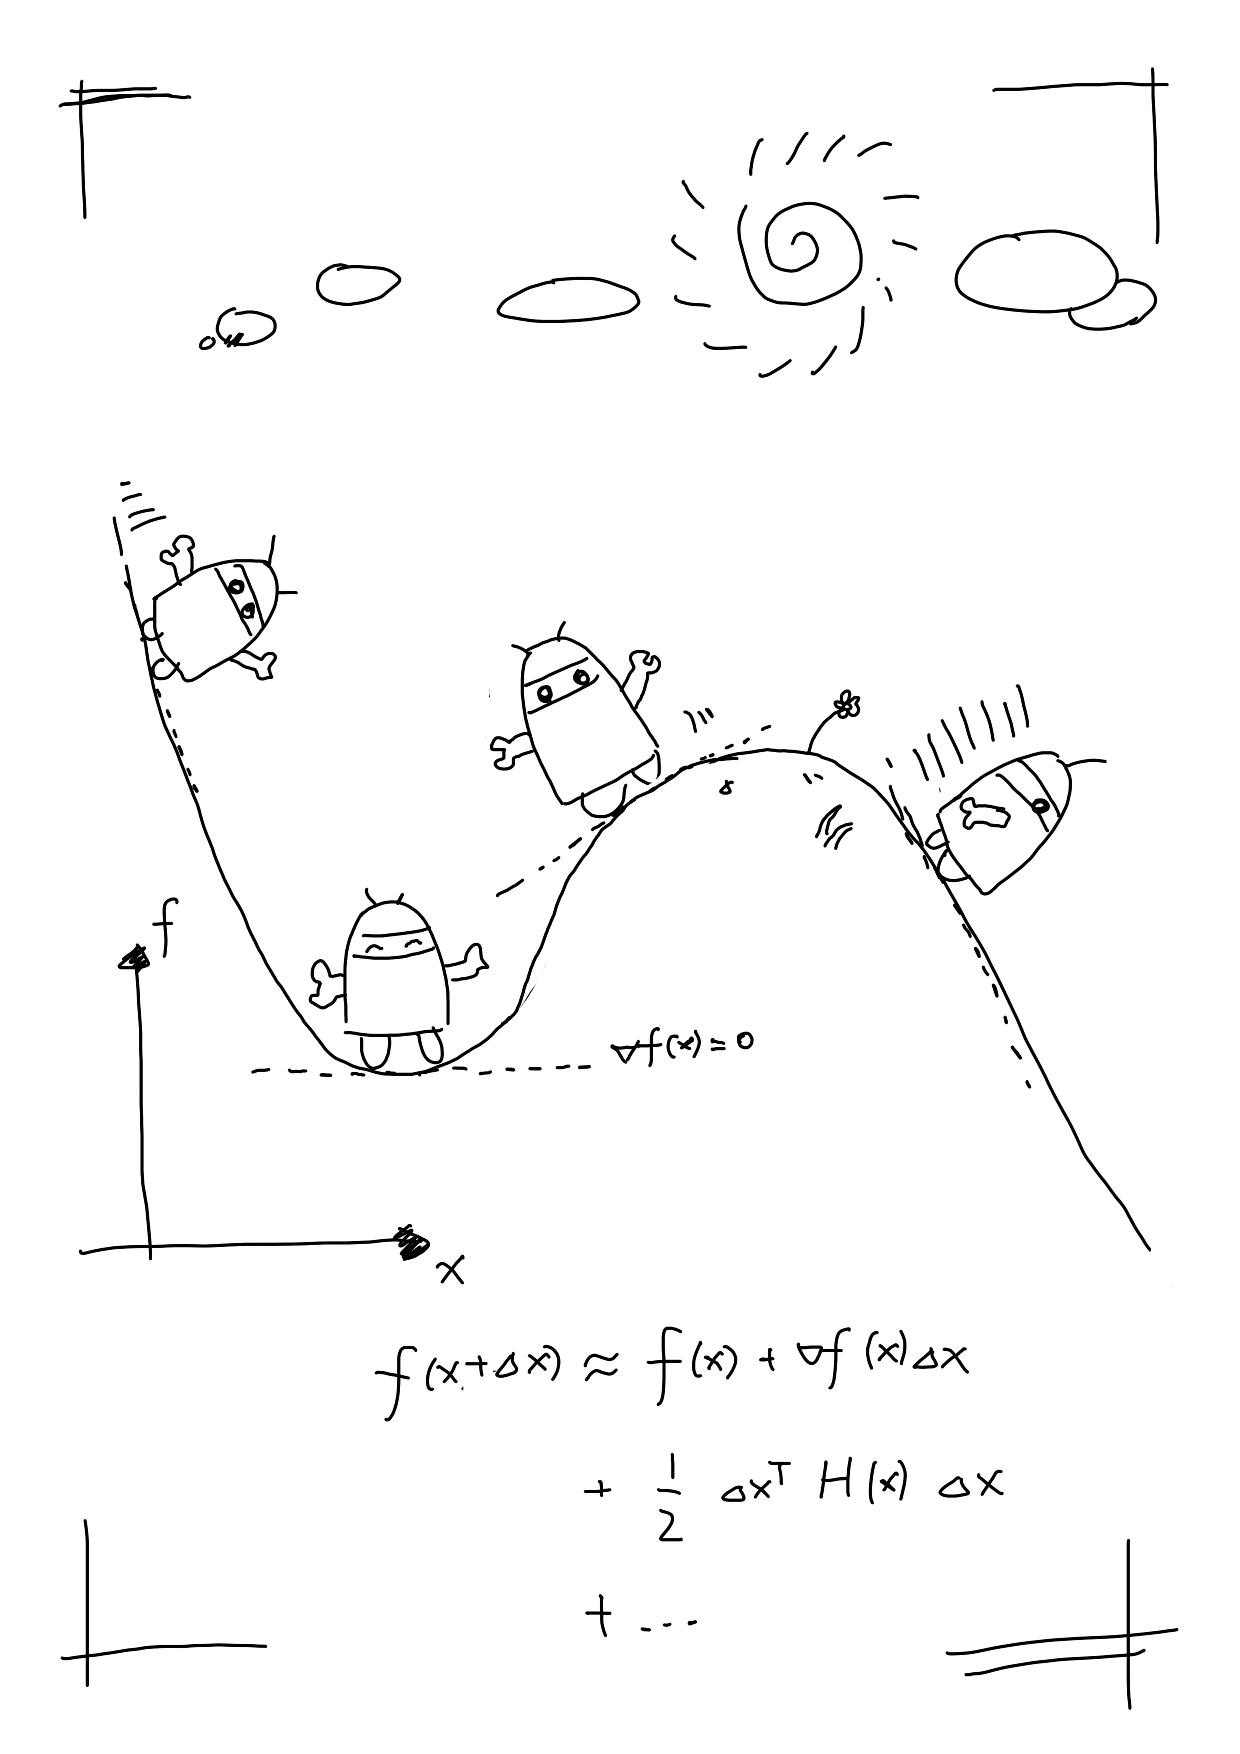
\includepdf{resources/other/ch6.pdf}

\newpage
\section{State Estimation}
\subsection{From Batch State Estimation to Least Square}
According to the previous sections, the SLAM process can be described by a discrete time motion and observation equations like \eqref{eq:slamproblem}:
\begin{equation}
\left\{ \begin{array}{l}
{\bm{x}_k} = \mathbf{f}\left( {{\bm{x}_{k - 1}},{\bm{u}_k}} \right) + \bm{w}_k\\
{\bm{z}_{k,j}} = \mathbf{h}\left( {{ \bm{y}_j},{ \bm{x}_k}}  \right)+ \bm{v}_{k,j}
\end{array} \right. .
\end{equation}

Through the knowledge in Lecture 4, we learned that $ \bm {x} _k $ is the pose of the camera, which can be described by $ \mathrm {SE} (3) $. As for the observation equation, we have already explained in Lecture 5, the pinhole camera model. In order to give readers a deeper impression of them, we may wish to discuss their specific parameterized form. First, the pose variable $\bm {x} _k $ can be expressed by $\bm {T} _k \in \mathrm {SE} (3) $. Second, the motion is related to the specific form of the input, but there is no particularity in visual SLAM (should be same as the case of ordinary robots and vehicles), we will not talk about it for the time being. The observation equation is given by the pinhole model. Assuming an observation of the road sign $ \bm {y} _j $ at $ \bm {x} _k $, corresponding to the pixel position on the image $ \bm {z} _ {k, j} $, then, observe The equation can be expressed as:
\begin{equation}
s \bm{z}_{k,j}= \bm{K} (\bm{R}_k {\bm{y}_j}+\bm{t}_k),
\end{equation}
where $ \bm {K} $ is the intrinsic matrix of the camera, and $s$ is the distance of pixels, which is also the third element of $ (\bm {R} _k {\bm {y} _j} + \bm {t} _k) $. If we use  transformation matrix $ \bm {T} _k $ to describe the pose, then the points $ \bm {y} _j $ must be described in homogeneous coordinates, and then converted to non-homogeneous coordinates afterwards. If you are not familiar with this process, please go back to the previous lectures.

Now, consider what happens when the data is affected by noise. In the motion and observation equations, we \textbf {usually} assume that the two noise terms $ \bm {w} _k, \bm {v} _ {k, j} $ satisfy a Gaussian distribution with zero mean, like this:
\begin{equation}
{\bm{w}_k} \sim \mathcal{N}\left( {\bm{0},{\bm{R}_k}} \right),{\bm{v}_k} \sim \mathcal{N}\left( {\bm{0},{{{\bm{Q}}}_{k,j}}} \right),
\end{equation}
where $ \mathcal {N} $ means Gaussian distribution, $ \bm{0} $ means zero mean, and $ \bm {R} _k, \bm {Q} _ {k, j} $ is the covariance matrix. Under the influence of these noises, we hope to infer the pose $ \bm {x} $ and the map $ \bm {y} $ from the noisy data $ \bm {z} $ and $ \bm {u} $ (and their probability density distribution), which constitutes a state estimation problem.

There are two ways to deal with this state estimation problem. Since these data come gradually over time in the SLAM process, intuitively, we should hold an estimated state at the current moment and then update it with new data. This method is called the \textbf {incremental} method, or \textbf{filtering}. For a long time in history, researchers have used filters, especially the extended Kalman filter (EKF) and its derivatives to solve it. The other way is to record the data into a file and looking for the best trajectory and map over all time. This method is called the \textbf {batch} estimation. In other words, we can put all the input and observation data from time 0 to $ k $ together, and ask, with such input and observation, how to estimate the entire trajectory and map from time 0 to $ k $?

These two different processing methods lead to many different estimation methods. In general, the incremental method only cares about the state estimation of the \textbf {current moment} $ \bm {x} _k $, but does not consider much about the previous state; relatively, the batch method can be used to get an optimized trajectory in larger time or space scope, which is considered to be superior to the traditional filters \textsuperscript {\cite {Strasdat2012}}, and has become the mainstream method of current visual SLAM. In extreme cases, we can let robots or drones collect data at all times and then bring it back to the computing center for unified processing, which is also the mainstream practice of SfM (Structure from Motion). Of course, in these cases the method is obviously not \textbf {real time}, which is not the most common application scenario of SLAM. So in SLAM, practical methods are usually some compromises. For example, we fix some historical trajectories and only optimize some trajectories close to the current moment, which leads to the \textbf {sliding window estimation} method to be described later.

In theory, the batch method is easier to introduce. At the same time, understanding the batch method also makes it easier to understand the incremental method. Therefore, in this section, we focus on the batch optimization method based on nonlinear optimization, and the Kalman filter and more in-depth knowledge will be discussed in the back-end chapter. Since the batch method is discussed, we will consider all the moments from time 1 to $ N $ and assume there are $ M $ map points. Define the robot pose and map coordinates at all times as:
\[
\bm{x}=\{ \bm{x}_1, \ldots, \bm{x}_N \}, \quad \bm{y} = \{\bm{y}_1, \ldots, \bm{y}_M \}.
\]
Similarly, $ \bm {u} $ without subscript is used for input at all times, and $ \bm {z} $ is used for observation data at all times. Then we say that the state estimation of the robot, from a probabilistic point of view, is to find the state $ \bm {x} , \bm{y}$ under the condition that the input data $ \bm {u} $ and the observation data $ \bm {z} $. Or, the conditional probability distribution of:
\begin{equation}
P( \bm{x},\bm{y} | \bm{z}, \bm{u}).
\end{equation}

In particular, when we do not know the control input and only have one image, that is, only considering the data brought by the observation equation, it is equivalent to estimating  the conditional probability distribution $ P (\bm {x}, \bm {y} | \bm { z}) $. Such a problem is also called Structure from Motion (SfM), that is, how to reconstruct the three-dimensional spatial structure from images only \textsuperscript {\cite {Agarwal2009}}.

To estimation the conditional pdf we use the Bayes equation to switch the variables:
\begin{equation}
P\left( { \bm{x},\bm{y}| \bm{z}, \bm{u}} \right) = \frac{{P\left( {\bm{z},\bm{u}|\bm{x},\bm{y}} \right)P\left( \bm{x}, \bm{y} \right)}}{{P\left( \bm{z},\bm{u}\right)}} \propto \underbrace{P\left(  { \bm{z},\bm{u}| \bm{x},\bm{y} } \right)}_{\text{likehood}} \underbrace{P\left( \bm{x},\bm{y} \right)}_{\text{prior}}.
\end{equation}

The left side is called \textbf {posterior probability}, and $ P (\bm {z} | \bm {x}) $ on the right is called \textbf {likelihood} (or likehood), and the other part is $ P (\bm {x}) $ is called \textbf {prior}. \textbf {It is normally difficult to find the posterior distribution directly (in nonlinear systems), but it is feasible to find an optimal point which maximize the posterior} (Maximize a Posterior, MAP):
\begin{equation}
{(\bm{x},\bm{y})^*}_{\mathrm{MAP}} = \arg {\mathop{\rm max}\nolimits} P \left( {\bm{x},\bm{y}|\bm{z},\bm{u}} \right) = \arg \max P(\bm{z},\bm{u}|\bm{x},\bm{y})P(\bm{x},\bm{y}).
\end{equation}

Please note that the denominator part of Bayes' rule has nothing to do with the state $ \bm {x}, \bm {y} $ to be estimated, so it can be just ignored. Bayes' rule tells us that solving the maximum posterior probability is \textbf {equivalent to the estimate the product of maximum likelihood and a priori}. Further, we can also say, I'm sorry, I don't know in prior where the robot pose or the map points are, and then there is no \textbf {prior}. Then, you can solve \textbf {Maximize Likelihood Estimation} (MLE):
\begin{equation}
{ (\bm{x},\bm{y})^*}_{\mathrm{MLE}} = \arg \max P( \bm{z},\bm{u}| \bm{x},\bm{y}).
\end{equation}

Intuitively speaking, likelihood refers to ``what observation data may be generated in the current pose''. Since we know the observation data, the maximum likelihood estimation can be understood as: ``\textbf{under what state is it most likely to produce the data currently observed}''. 

\subsection{Introduction to Least Squares}
Now we have a formulated the state estimation problem into a MAP/MLE problem, and the next question is how to solve it. Under the assumption of Gaussian distribution, we can have a simpler form of the maximum likelihood problem. Looking back at the observation model, for a certain kind of observation, we have:
\[
{\bm{z}_{k,j}} = h\left( {{ \bm{y}_j},{ \bm{x}_k}} \right)+ \bm{v}_{k, j},
\]
Since we assume the noise item is gaussian, which means ${\bm{v}_k} \sim \mathcal{N}\left( {\bm{0},{{{\bm{Q}}}_{k,j}}} \right)$, so the conditional probability of the observation data is:
\[
P( \bm{z}_{j,k} | \bm{x}_k, \bm{y}_j) = N\left( h(\bm{y}_j, \bm{x}_k), \bm{Q}_{k,j} \right),
\]
which is, of course, still a Gaussian distribution. Now let's considering to solve the maximum likelihood estimation under this single observation. 

We can rewrite this maximum problem into a \textbf{minimium of negative logarithm} one for Gaussian distributions since they have better mathematical forms under negative logarithm. Consider an arbitrary multi-dimensional Gaussian distribution $\bm{x} \sim \mathcal{N}(\bm{\mu}, \bm{\Sigma})$, its probability density function expansion form is:
\begin{equation}
	P\left( \bm{x} \right) = \frac{1}{{\sqrt {{{(2\pi )}^N}\det (\bm{\Sigma} )} }}\exp \left( {-\frac{1}{2}{{\left( {\bm{x}-\bm{\mu}} \right)}^\mathrm{T}}{ \bm{\Sigma} ^ {-1}}\left( {\bm{x}-\bm{\mu}} \right)} \right).
\end{equation}
Taking the negative logarithm of both sides:
\begin{equation}
	-\ln \left( {P\left( \bm{x} \right)} \right) = \frac{1}{2}\ln \left( {{{\left( {2\pi} \right )}^N}\det \left( \bm{\Sigma} \right)} \right) + \frac{1}{2}{\left( {\bm{x}-\bm{\mu}} \right)^\mathrm{T}}{\bm{\Sigma} ^{-1}}\left( {\bm{x}-\bm{\mu}} \right).
\end{equation}
Because the logarithm function is monotonically increasing, maximizing the original function is equivalent to minimizing the negative logarithm. When minimizing $\bm{x}$ in the above formula, the first term has nothing to do with $\bm{x}$ and can be omitted. Therefore, as long as the quadratic term on the right is minimized, the maximum likelihood estimate of the state is obtained. Substituting into the SLAM observation model, it is equivalent to finding such a solution:
\begin{equation}
	\begin{aligned}
		(\bm{x}_k,\bm{y}_j)^* &= \arg \max \mathcal{N}(h(\bm{y}_j, \bm{x}_k), \bm{Q }_{k,j}) \\ &= \arg \min \left( {{{\left( {{ \bm{z}_{k,j}}-h\left( {{\bm{x }_k},{\bm{y}_j}} \right)} \right)}^\mathrm{T}} \bm{Q}_{k,j}^{-1}\left( {{\ bm{z}_{k,j}}-h\left( {{\bm{x}_k},{\bm{y}_j}} \right)} \right)} \right).
	\end{aligned}
\end{equation}

We found that this equation is equivalent to a quadratic form that minimizes the noise term (i.e., the error). This quadratic form is called \textbf{Mahalanobis distance}. It can also be regarded as the Euclidean distance ($\mathcal{L}_2$-norm) weighted by $\bm{Q}_{k,j}^{-1}$, where $\bm{Q}_{k,j} ^{-1}$ is also called the \textbf{information matrix}, which is extacly the \textbf{inverse} of the Gaussian  \textbf{covariance matrix}.

Now we put all the observations together. It is usually assumed that the inputs and observations at each time are independent of each other, which means that each input is independent, each observation is independent, and input and observation are also independent. So we can factorize the joint distribution like this:
\begin{equation}
	P\left( {\bm{z},\bm{u}|\bm{x},\bm{y}} \right) = \prod\limits_k {P\left( {{\bm{u}_k }|{\bm{x}_{k-1}},{\bm{x}_k}} \right)} \prod\limits_{k,j} {P\left( {{\bm{z} _{k,j}}|{\bm{x}_k},{\bm{y}_j}} \right)},
\end{equation}

It shows that we can handle the movement and observation at each moment independently. Let's define the error between the model and real data: 
\begin{equation}
	\begin{array}{l}
		{\bm{e}_{u,k}} = {\bm{x}_k}-f\left( {{\bm{x}_{k-1}},{\bm{u}_k} } \right)\\
		{\bm{e}_{z,j,k}} = {\bm{z}_{k,j}}-h\left( {{\bm{x}_k},{\bm{y} _j}} \right),
	\end{array}
\end{equation}
Then, minimizing the Mahalanobis distance between the estimated value at all times and the measurements from sensors is equivalent to finding the maximum likelihood estimation. The negative logarithm allows us to turn the product into a summation:
\begin{equation}
	\label{eq:least-square}
	\min J (\bm{x},\bm{y}) = \sum\limits_k {\bm{e}_{u,k}^\mathrm{T} \bm{R}_k^{-1} {\bm{e}_{u,k}}} + \sum\limits_k {\sum\limits_j {\bm{e}_{z,k,j}^\mathrm{T} \bm{Q}_ {k,j}^{-1}{\bm{e}_{z,k,j}}}}.
\end{equation}
In this way, a \textbf{least square problem} is obtained with the same solution as the MLE problem. Intuitively speaking, due to the presence of noise, when we substitute the estimated trajectory and map into the SLAM motion and observation models, they will not be perfectly fit. What shall we do at this time? We perform \textbf{fine-tuning} on the estimated value of the state, so that the overall error is reduced. Of course, finally we will reach a (local) \textbf{minimum value}. This is a typical nonlinear optimization process.

Observing the formula \eqref{eq:least-square} carefully, we find that the least squares problem in SLAM has some specific structures:

\begin{itemize}
	\item First of all, the objective function of the whole problem consists of many (weighted) error quadratic forms. Although the dimensionality of the overall state variable is very high, each error term is simple and is only related to one or two state variables. For example, the motion error is only related to $\bm{x}_{k-1}, \bm{x}_k$, and the observation error is only related to $\bm{x}_k, \bm{y}_j$. This relationship will give a \textbf{sparse} least square problem, which we will investigate further in the backend chapter.

	\item Secondly, if you use Lie algebra to represent the increment, the problem is the least squares problem of \textbf{unconstrained}. However, if the rotation matrix/transformation matrix is ​​used to describe the pose, the constraint of the rotation matrix itself will be introduced, that is, $\mathrm{st}\ \bm{R}^\mathrm{T} \bm{R} = \bm{I}$ and $\det (\bm{R})=1$ need to be added to the problem. Additional constraints can make optimization more difficult. 

	\item Finally, we used a quadratic metric error, which is exactly the $\mathcal{L}_2-$norm. The information matrix is used as the weights of each elemnents. For example, if an observation is very accurate, the covariance matrix will be ``small'' and the information matrix will be ``large'', so this error term will have a higher weight than the others in the whole problem. We will see some drawbacks of the $\mathcal{L}_2$ error later.
\end{itemize}

Now, we introduce how to solve this least squares problem, which requires some \textbf{basic knowledge of nonlinear optimization}. In particular, we want to discuss how to solve such a general unconstrained nonlinear least squares problem. In the following lectures, we will make extensive use of the results of this lecture and discuss in detail its application in the front and back ends of SLAM.

